\documentclass[a4paper, 12pt, final, garamond]{book}
\usepackage{cours-preambule}

\raggedbottom

\makeatletter
\renewcommand{\@chapapp}{Programme de kh\^olle -- semaine}
\makeatother

\begin{document}
\setcounter{chapter}{12}

\chapter{Du 03 au 06 janvier}

\section{Cours et exercices}
\section*{Électrocinétique chapitre 6 -- Oscillateurs en RSF}
\begin{enumerate}[label=\Roman*]
    \item \textbf{Introduction}~: rappel oscillateurs, méthode des complexes,
        notion de résonance et bande passante.
    \item \textbf{Exemple électrique~: circuit RLC série en RSF}~: présentation,
        étude de l'intensité (amplitude complexe, amplitude réelle et maximum,
        phase, influence de $Q$), étude de la tension (amplitude complexe,
        amplitude réelle et condition de résonance, phase).
    \item \textbf{Exemple mécanique~: ressort horizontal en RSF}~: présentation,
        étude de l'élongation (amplitude d'élongation complexe, amplitude réelle
        et condition de résonance), résonance en vitesse.
\end{enumerate}

\section*{Électrocinétique chapitre 7 -- Filtrage linéaire}
\begin{enumerate}[label=\Roman*]
    \item \textbf{Signaux périodiques}~: période, moyenne, valeur efficace.
    \item \textbf{Décomposition en série de Fourier}~: théorème de
        \textsc{Fourier}, analyse spectrale, relation de \textsc{Parseval}.
    \item \textbf{Filtrage linéaire}~: introduction, fonction de transfert d'un
        filtre, effet d'un filtre sur un signal périodique.
    \item \textbf{Description d'un filtre}~: gain et gain en décibels, diagramme
        de \textsc{Bode} (définition, exemple, asymptotes, lecture), filtres
        moyenneurs dérivateurs et intégrateurs.
    \item \textbf{Filtres d'ordre 1}~: RC sur C~: passe-bas, RC sur R~:
        passe-haut.
    \item \textbf{Filtres d'ordre 2}~: RLC sur C~: passe-bas d'ordre 2, RLC sur R~:
        passe-bande.
    \item \textbf{Filtres en cascade}~: nécessité d'adaptation d'impédance.
\end{enumerate}

% \section{Cours uniquement}

\section{Questions de cours possibles}
\begin{enumerate}
    \item Étude de la résonance en \textbf{intensité} pour le circuit RLC série
        en RSF~: introduire le système, déterminer l'amplitude complexe
        $\Iu(\w)$ sous forme canonique, déterminer l'amplitude réelle $I(\w)$ et
        la pulsation de résonance, tracer l'allure de l'amplitude réelle.

    \item À partir de $\Iu(\w) = 
        \dfrac{E_0/R}{\sqrt{1 + Q^2\left( \dfrac{\w}{\w_0} - \dfrac{\w_0}{\w}
        \right)^2}}$, déterminer les valeurs $\w_1$ et $\w_2$ donnant
        les limites de la bande passante et exprimer la largeur de la
        bande passante en fonction de facteur de qualité.

    \item Étude de la résonance en \textbf{élongation} pour le ressort
        horizontal en RSF~: introduire le système, déterminer l'amplitude
        complexe $\Xu(\w)$ sous forme canonique, déterminer l'amplitude réelle
        $X(\w)$ et la pulsation de résonance en explicitant la condition de
        résonance, tracer l'allure de l'amplitude réelle.

    \item Filtre passe-bas d'ordre 1, RC série sur C~: présenter le système
        réel, le système en RSF complexe, déterminer sa fonction de transfert,
        son gain en décibels, l'évolution de sa phase et tracer son diagramme de
        \textsc{Bode} en détaillant les asymptotes à basses et hautes fréquences
        pour le gain.

    \item Filtre passe-haut d'ordre 1, RC série sur R~: présenter le système
        réel, le système en RSF complexe, déterminer sa fonction de transfert,
        son gain en décibels, l'évolution de sa phase et tracer son diagramme de
        \textsc{Bode} en détaillant les asymptotes à basses et hautes fréquences
        pour le gain.

    \item Comportements intégrateur et dérivateur~: définir les comportements
        intégrateur et dérivateur d'un filtre, donner les formes canoniques
        des filtres passe-bas et passe-haut d'ordre 1, et démontrer leur
        comportement intégrateur ou dérivateur.

    \item Filtre passe-bas d'ordre 2, RLC série sur C~: présenter le système
        réel, le système en RSF complexe, déterminer sa fonction de transfert,
        son gain en décibels, l'évolution de sa phase et tracer son diagramme de
        \textsc{Bode} en détaillant les asymptotes à basses et hautes fréquences
        pour le gain.

    \item Filtre passe-bande d'ordre 2, RLC série sur R~: présenter le système
        réel, le système en RSF complexe, déterminer sa fonction de transfert,
        son gain en décibels, l'évolution de sa phase et tracer son diagramme de
        \textsc{Bode} en détaillant les asymptotes à basses et hautes fréquences
        pour le gain.

    \item Refaire l'exercice~:
\end{enumerate}
\begin{NCexem}[]{Exercice}
    On considère le circuit ci-contre, avec $R = \SI{1.0}{k\Omega}$ et $L =
    \SI{10}{mH}$, donnant le diagramme de \textsc{Bode} ci-dessous~:

    \begin{minipage}{0.60\linewidth}
        \begin{enumerate}
            \item Sans utiliser le diagramme de \textsc{Bode}, quelle est la
                nature du filtre~?
            \item Déterminer sa fonction de transfert et l'écrire sous la forme
                \[\ul{H}(\jj\w) = H_0 \frac{\jj\dfrac{\w}{\w_c}}{1 +
                \jj\dfrac{\w}{\w_c}}\] avec $H_0$ et $\w_c$ des constantes à
                préciser.
            \item On considère une tension d'entrée $u_e(t)$ somme de 3
                harmoniques de mêmes amplitudes, de mêmes phases initiales, mais
                de fréquences respectives $f_1 = \SI{100}{Hz}$, $f_2 =
                \SI{1}{kHz}$ et $f_3 = \SI{100}{kHz}$. Donner le spectre de
                sortie.
        \end{enumerate}
    \end{minipage}
    \hfill
    \begin{minipage}{0.35\linewidth}
        \begin{center}
            \hspace{10pt}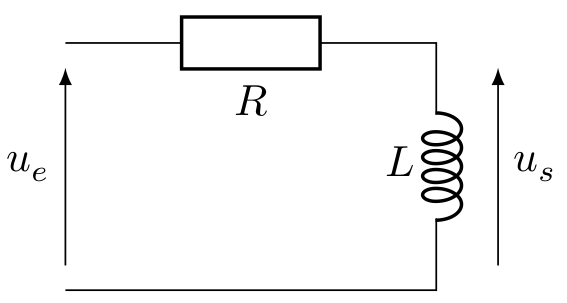
\includegraphics[width=\linewidth]{filtrebob_plain}
        \end{center}
        \begin{center}
            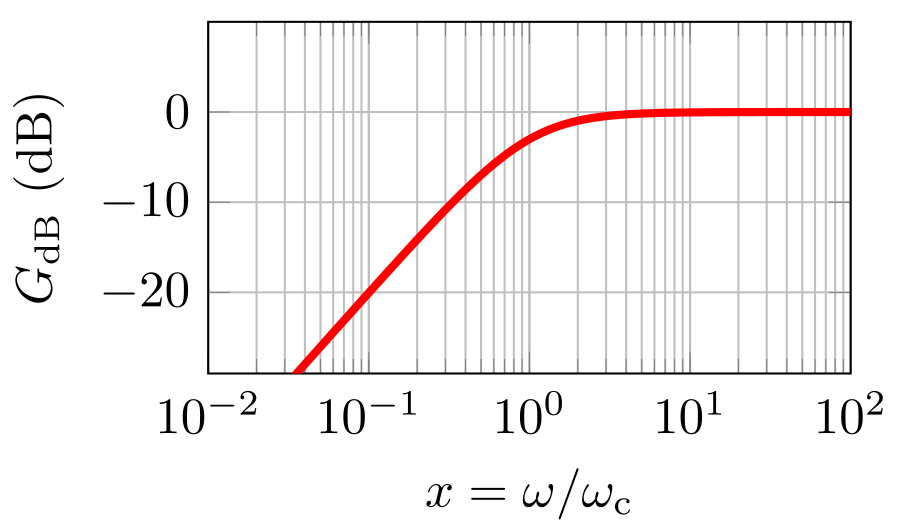
\includegraphics[width=\linewidth]{filtrebob_bode}
        \end{center}
    \end{minipage}
\end{NCexem}
\end{document}
